%%%%%%%%%%%%%%%%%%%%%%%%%%%%%%%%%%%%%%%%%%%%%%%
% Template per Elaborato di Laurea
% DISI - Dipartimento di Ingegneria e Scienza dell’Informazione
%
% update 2015-09-10
%
% Per la generazione corretta del 
% pdflatex nome_file.tex
% bibtex nome_file.aux
% pdflatex nome_file.tex
% pdflatex nome_file.tex
%%%%%%%%%%%%%%%%%%%%%%%%%%%%%%%%%%%%%%%%%%%%%%%

% formato FRONTE RETRO
\documentclass[epsfig,a4paper,11pt,titlepage,twoside,openany]{book}
\usepackage{epsfig}
\usepackage{plain}
\usepackage{setspace}
\usepackage[paperheight=29.7cm,paperwidth=21cm,outer=1.5cm,inner=2.5cm,top=2cm,bottom=2cm]{geometry} % per definizione layout
\usepackage{titlesec} % per formato custom dei titoli dei capitoli


%%%%%%%%%%%%%%
% supporto lettere accentate
%
%\usepackage[latin1]{inputenc} % per Windows;
\usepackage[utf8x]{inputenc} % per Linux (richiede il pacchetto unicode);

\singlespacing
\usepackage[italian]{babel}

\begin{document}

  % nessuna numerazione
  \pagenumbering{gobble} 
  \pagestyle{plain}

\thispagestyle{empty}

\begin{center}
  \begin{figure}[h!]
    \centerline{
\psfig{file=logo_unitn_black_center.eps,width=0.6\textwidth}}
  \end{figure}

  \vspace{2 cm} 

  \LARGE{Dipartimento di Ingegneria e Scienza dell’Informazione\\}

  \vspace{1 cm} 
  \Large{Corso di Laurea in\\
   Informatica}

  \vspace{2 cm} 
  \Large\textsc{Elaborato finale\\} 
  \vspace{1 cm} 
  \Huge\textsc{Titolo\\}
  \Large{\it{Sottotitolo (alcune volte lungo - opzionale)}}


  \vspace{2 cm} 
  \begin{tabular*}{\textwidth}{ c @{\extracolsep{\fill}} c }
  \Large{Supervisore} & \Large{Laureando}\\
  \Large{Martin Hanczyc}& \Large{Carlotta Porcelli}\\
  \end{tabular*}

  \vspace{2 cm} 

  \Large{Anno accademico 2015/2016}
  
\end{center}


  \clearpage
 
%%%%%%%%%%%%%%%%%%%%%%%%%%%%%%%%%%%%%%%%%%%%%%%%%%%%%%%%%%%%%%%%%%%%%%%%%%
%% Nota
%% Sezione Ringraziamenti opzionale
%%%%%%%%%%%%%%%%%%%%%%%%%%%%%%%%%%%%%%%%%%%%%%%%%%%%%%%%%%%%%%%%%%%%%%%%%%

  \thispagestyle{empty}

\begin{center}
  {\bf \Huge Ringraziamenti}
\end{center}

\vspace{4cm}


\emph{
 A mamma e papà, per esserci sempre stati
}

  \clearpage
  \pagestyle{plain} % nessuna intestazione e pie pagina con numero al centro

  
  % inizio numerazione pagine in numeri arabi
  \mainmatter

%%%%%%%%%%%%%%%%%%%%%%%%%%%%%%%%%%%%%%%%%%%%%%%%%%%%%%%%%%%%%%%%%%%%%%%%%%
%% Nota:
%% Si ricorda che il numero massimo di facciate e' 30.
%% Nel conteggio delle facciate sono incluse 
%%   indice
%%   sommario
%%   capitoli
%% Dal conteggio delle facciate sono escluse
%%   frontespizio
%%   ringraziamenti
%%   allegati    
%%%%%%%%%%%%%%%%%%%%%%%%%%%%%%%%%%%%%%%%%%%%%%%%%%%%%%%%%%%%%%%%%%%%%%%%%%

    % indice
    \tableofcontents
    \clearpage
      
    % gruppo per definizone di successione capitoli senza interruzione di pagina
   	%\begingroup
      % nessuna interruzione di pagina tra capitoli
      % ridefinizione dei comandi di clear page
      %\renewcommand{\cleardoublepage}{} 
      %\renewcommand{\clearpage}{} 
      % redefinizione del formato del titolo del capitolo
      % da formato
      %   Capitolo X
      %   Titolo capitolo
      % a formato
      %   X   Titolo capitolo
      
      \titleformat{\chapter}
        {\normalfont\Huge\bfseries}{\thechapter}{1em}{}
        
      \titlespacing*{\chapter}{0pt}{0.59in}{0.02in}
      \titlespacing*{\section}{0pt}{0.20in}{0.02in}
      \titlespacing*{\subsection}{0pt}{0.10in}{0.02in}
      
      % sommario
      \chapter*{Sommario} % senza numerazione
\label{sommario}
\addcontentsline{toc}{chapter}{Sommario}% da aggiungere comunque all'indice

\textbf{Contesto}
\\Gli studi presentati in questa tesi sono stati svolti presso il laboratorio di Biologia Artificiale del CIBIO - Centre for Integrative Biology dell'Università di Trento che partecipa al progetto EVOBLISS: un progetto di ricerca europeo a cui collaborano anche i laboratori di altre cinque università europee. Questo progetto combina gli approcci scientifici della robotica, dell'intelligenza artificiale, della chimica e della microbiologia. Lo scopo finale è quello di produrre una piattaforma robotica facilmente utilizzabile e personalizzabile per l'evoluzione artificiale di nuovi materiali. 
\\Il prodotto su cui si è lavorato è EvoBot, un robot in grado di gestire liquidi e di fornire riscontri in tempo reale su sistemi da esso stesso creati. Lo scopo del progetto è quello di riprodurre caratteristiche base degli organismi viventi, nello specifico ci si è soffermati sul movimento, studiato in un sistema chimico. Varie sostanze chimiche vengono utilizzate in strutture che si comportano come sistemi viventi. I sistemi vengono alimentati con opportuni nutrienti e viene osservato il loro comportamento, nello specifico il movimento, caratteristica fondamentale di un organismo vivente. 
\\Lo studio dei risultati è stato eseguito per mezzo di un software di computer vision con l'ausilio di EvoBot per l’esecuzione vera e propria degli esperimenti. La particolarità di EvoBot sta nel permettere all'utente un'interazione continua ed in tempo reale con l'esperimento in corso.\cite{introd-robot} Inoltre, utilizzare un robot per la gestione degli esperimenti ha permesso di diminuire, quasi annullare, l'incertezza e la variazione tra gli esperimenti causata dalla manualità. 
\\EvoBot è un robot che unisce elementi delle stampanti 3D con quelli della robotica modulare per fornire a chimici e a ricercatori nel campo della vita (a livello chimico) artificiale, uno strumento estendibile basato su una piattaforma open source di robotica per il trattamento di liquidi.
\begin{wrapfigure}{r}{0.5\textwidth}
\begin{center}
	  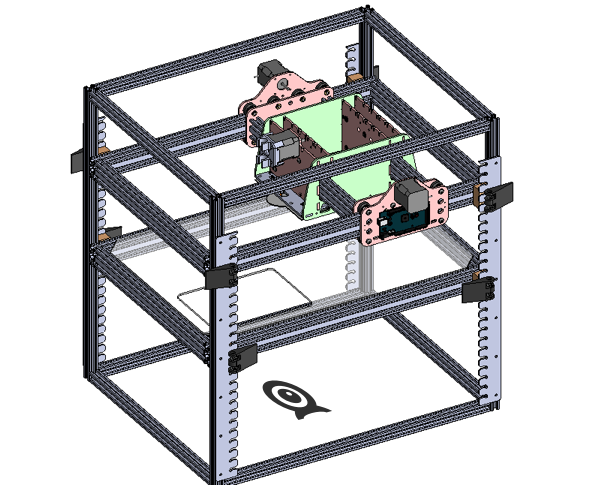
\includegraphics[width=0.48\textwidth]{immagini/observational-layer.png}
\end{center}
	 \caption{La struttura completa del robot}
	\end{wrapfigure} 
Il robot, come schematizzato in Figura 1, è composto da tre strati: dal basso si ha lo strato dell'\emph{osservazione}, all'interno del quale è posta una webcam statica utilizzata sia per la registrazione degli esperimenti, sia per l'interazione con il robot. Il secondo strato, degli \emph{esperimenti}, è composto da una superficie di vetro trasparente sulla quale vengono sistemati i recipienti richiesti dagli specifici esperimenti. L'ultimo strato, lo strato dell'\emph{attuazione} è composto dalla testa del robot. Questa struttura si muove a livello orizzontale lungo il piano. La testa è composta da circuiti stampati costituiti da connettori a molla per l'inserimento di moduli specifici. Ad oggi esiste soltanto il modulo siringa ma si prevede nel breve futuro, la costruzione di altri moduli come sensori di pH e di temperatura. 
\\Il modulo siringa ha due gradi di movimento verticale. Ogni modulo è composto di un motore passo-passo lineare per il movimento dello stantuffo, \emph{plunger}, e di un meccanismo a rocchetto e cremagliera con un secondo motore passo-passo per il movimento del corpo della siringa. La siringa può essere facilmente sostituita dando all'utente l'opportunità di utilizzare siringhe con specifiche differenti in base alle necessità del singolo esperimento. Le siringhe sono la componente di EvoBot che gli permette la gestione di sostanze liquide. 
\\Il robot può essere controllato manualmente o con programmi appositamente sviluppati con le API messe a disposizione da EvoBot. Per controllare manualmente EvoBot si utilizza Printrun \cite{printrun}, una \emph{3D printing host suite}  opensource, con la quale, attraverso dei codici G standard, si controlla il movimento della testa del robot e con dei codici M speciali si controlla il movimento delle siringhe e degli stantuffi.

\textbf{L'esperimento}
\begin{wraptable}{r}{0.5\textwidth}
\caption{Spazio multiparametrico degli esperimenti}
\begin{center}
\begin{tabular}{l|l|l|l}
\backslashbox{\textbf{molarità}}{\textbf{ph}} & \textbf{11} & \textbf{12} & \textbf{13} \\ \hline
\textbf{20mM} &  &   &   \\ \hline
\textbf{10mM} &    &   &   \\ \hline
\textbf{5mM}  &    &  &  \\ \hline
\end{tabular}
\end{center}
\end{wraptable}
Una delle proprietà fondamentali degli organismi viventi è l'abilità di sentire e rispondere ai cambiamenti dell'ambiente tramite il movimento. 
Una cellula che percepisce delle molecole solubili può muoversi lungo il gradiente di concentrazione creato da queste fino a raggiungere la sorgente oppure allontanarsi da questa nel caso in cui le sostanze rilasciate siano repellenti o tossine.
Il movimento preso in analisi è un movimento di \emph{chemiotassi}. La \emph{chemiotassi} può essere di tipo positivo in caso di avvicinamento alla sorgente e di tipo negativo in caso di allontanamento. Lo studio è stato svolto sul movimento chemiotattico positivo promosso da una \emph{droplet} di decanolo in soluzione acquosa di Acido decanoico $(CH_{3}(CH_{2})_8COOH)$ lungo il gradiente di concentrazione creato dall'aggiunta di Cloruro di sodio. Il movimento di auto-avanzamento di oggetti non biologici simula il comportamento chemiotattico di cellule viventi. 
\\Una \emph{droplet} posizionata sulla superficie di un substrato, può muoversi quando la superficie sottostante cambia il proprio motivo in modo asimmetrico creando una differenza nella tensione interfacciale tra il margine anteriore e il margine posteriore della droplet. 
Inoltre una \emph{droplet} può rompere la simmetria attraverso una reazione chimica accoppiata che avviene all'interfaccia tra la droplet e la soluzione circostante. La reazione chimica produce una rottura della simmetria dovuta all'accumulo e al rilascio di prodotti che inducono la droplet a muoversi attraverso la soluzione acquosa.\cite{selfpropelled}
\\In particolare, e' stata analizzata la dipendenza parametrica della risposta chemiotattica della droplet al variare della concentrazione e del pH di Sodio Decanoato in rapporto alla forza del gradiente di concentrazione di $NaCl$ $3.5M$. 
Lo spazio multiparametrico utilizzato ha previsto l'esecuzione di ripetizioni di ognuno dei nove esperimenti composti come in tabella 1.

\textbf{Tecniche utilizzate}
\\Analizzando i diversi comportamenti della droplet nei vari esperimenti eseguiti e tenendo in considerazione che l'obiettivo di tale studio è quello di fare in modo che questa si muova velocemente e in maniera precisa lungo un percorso ipotizzato, si è cercata la combinazione ``migliore" dei parametri sperimentali che permettesse alla droplet di avvicinarsi il più possibile e nel minor tempo al punto in cui il sale è stato posto. 
\begin{wrapfigure}{r}{0.5\textwidth}
\begin{center}
	  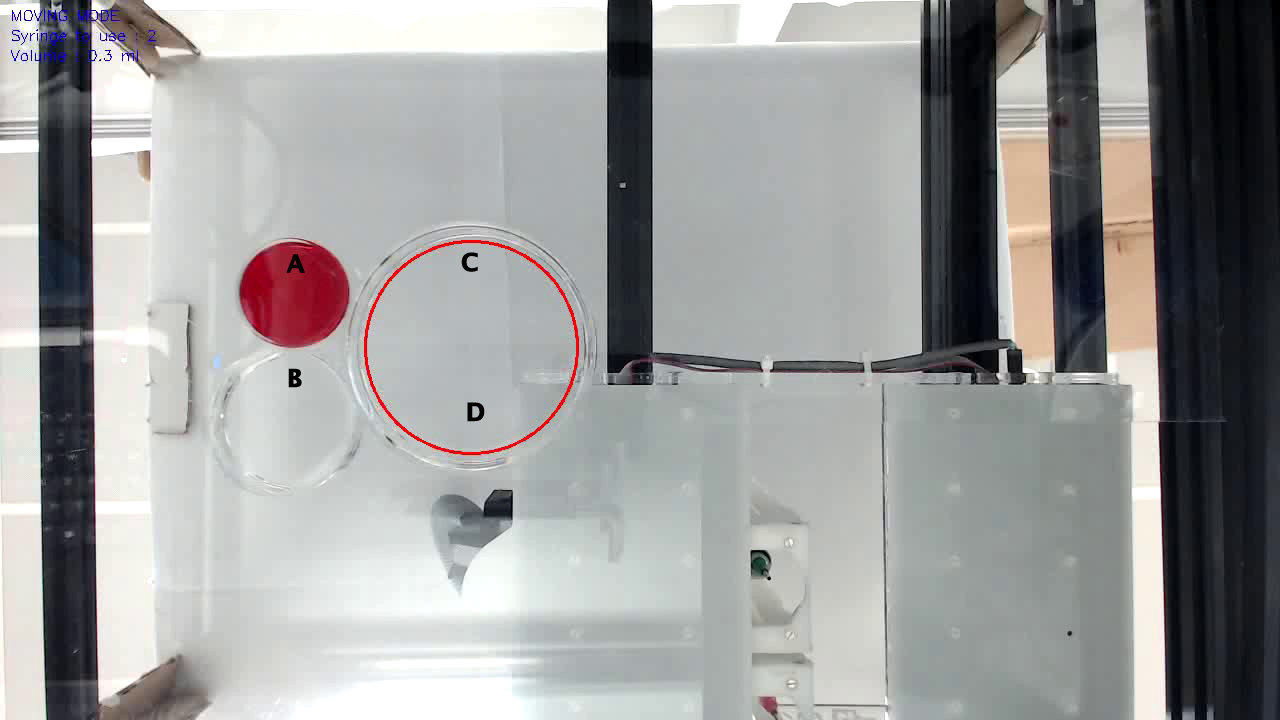
\includegraphics[width=0.3\textwidth]{immagini/exp1.jpg}
\end{center}
	 \caption{Disposizione dell'esperimento}
\end{wrapfigure} 
Lo studio di questo movimento di chemiotassi, ci aiuterà a comprendere e a riprodurre le dinamiche di movimento delle cellule viventi. 
L'esperimento precedentemente descritto, è stato eseguito per mezzo del programma appositamente sviluppato, utilizzando le API di EvoBot e sfruttando funzioni avanzate della libreria OpenCV. 
Per portare a termine l'intero esperimento occorre completare tre fasi: preparazione, raccolta dati ed elaborazione dati. 
Nella preparazione si utilizza la disposizione come in Figura 2 e un protocollo caratterizzato dai seguenti passaggi fondamentali:
\\1. Limitazione dell'area di interesse: attraverso l’apposita interfaccia è possibile disegnare un cerchio attorno alla Petri dish, permettendo così di non considerare tutto ciò che si trova all'esterno di questo limite virtuale dal programma.
\\2. Gestione del decanolo: prelevare $50\mu L$ di decanolo utilizzando una siringa delle due a disposizione, si raggiunge il pozzetto A e si fa scendere il corpo della siringa per prelevare la quantità di decanolo richiesta. Rilasciare $30\mu L$ di decanolo posizionando la siringa precedentemente caricata sopra la Petri dish in posizione C, si rilascia il decanolo. 
\\3. Gestione del sale: prelevare $500\mu L$ di NaCl utilizzando l'altra siringa, si raggiunge il pozzetto B e si eseguono le stesse azioni del punto 2, prelevando questa volta il sale. Immettere $200\mu L$ di NaCl posizionando la siringa attualmente in uso sopra la Petri dish in posizione D, si rilascia il sale. 
\\Tramite l'utilizzo della webcam statica e la libreria di OpenCV, il programma permette di tracciare passo-passo i movimenti della droplet, fino a 30 al secondo. \\Nel nostro caso ci siamo soffermati ad osservare se ci fosse un movimento della droplet verso il sale e si è cercato di capire in che ambiente questo risultasse più veloce e più preciso. Nella raccolta dei dati il programma si serve del salvataggio di questi su di un file \emph{.csv}. Un esempio di questo file è disponibile nella tabella sottostante. 
\begin{center}
\begin{tabular}{lllllll}
X salt & Y salt & X droplet Start & Y droplet Start & X droplet End & Y droplet End & time(s) \\
\hline
405    & 418    & 378             & 300             & 425           & 434           & 88  
\end{tabular}
\end{center}
I file prodotti durante la raccolta dati, vengono successivamente presi in carico da un altro programma che ha il compito di analizzare queste rilevazioni col fine di generare un unico file contenente dati e metadati dei singoli esperimenti. La colonna più importante del file generato è quella che prende il nome di ``k". Questo coefficiente indica la precisione con cui la droplet si avvicina al sale ed è definita come:
\begin{equation} 	
	k := \frac { d(C,B) }{ d(A,C) }
\end{equation}
Dove A rappresenta il punto in cui la droplet viene trovata all'inizio del tracking, B quello in cui viene posizionato il sale, C dove la droplet si trova ad esperimento concluso, ed infine $d$ calcola la distanza euclidea tra i punti in questione. 
\\Possiamo assumere che più $d(C,B)$ tende a zero, più l'esperimento è preciso; da questo si evince che avere un $k$ tendente a zero è indice di successo. Una volta ottenuti tutti i $k$, mantenendo costante il $pH$ e le molarità, si vanno a calcolare tutti i $k$ medio per ogni singolo ambiente. L'ambiente rappresentato dal minor $k$ medio è quello che permette alla droplet di raggiungere il sale in maniera precisa e veloce. \\

\textbf{Risultati raggiunti}
\\I dati hanno dimostrato che nelle soluzioni $10mM$ e $5mM$ la droplet compie dei percorsi più lunghi, arrivando molto vicina al punto di inserimento del sale. Tuttavia, nelle soluzioni $20mM$ si osservano dei movimenti più brevi, come se la droplet facesse fatica a riconoscere il gradiente del sale compiendo un movimento minimo. Bisogna tenere in considerazione che questo movimento può essere influenzato da flussi di aria capaci di creare dei moti convettivi all'interno del sistema. I moti possono agire come forza contraria alla direzione del movimento. 
\begin{wraptable}{r}{0.55\textwidth}
\caption{Tabella riassuntiva}
%\begin{center}
\begin{tabular}{l|lll}
\backslashbox{\textbf{molarità}}{\textbf{ph}} & \textbf{11} & \textbf{12} & \textbf{13} \\ \cline{1-4} 
\textbf{20mM} & 2,013 & 3,357 & 4,742 \\ 
\textbf{10mM} & 0,373  & 0,504 & 0,592 \\ \cline{2-2}
\multicolumn{1}{l|}{\textbf{5mM}} & \multicolumn{1}{l|}{0,209} & 0,67  & 0,327 \\ \cline{2-2}
\end{tabular}
%\end{center}
\end{wraptable}
\\Tuttavia queste ipotesi potranno essere confermate attraverso la ripetizione di un maggior numero di esperimenti.
Nella tabella riassuntiva 2 sono stati raccolti tutti i valori medi di ogni combinazione. Come si può osservare il coefficiente di precisione migliore si ha nella soluzione $5mM$ con $pH11$. Inoltre, le soluzioni $20mM$ hanno i coefficienti maggiori tra tutte, sinonimo di una minore precisione della droplet nel raggiungimento della sorgente di sale.





















   	
%%%%%%%%%%%%%%%%%%%%%%%%%%%%%%%%%%%%%%%%%%%%%%%%%%%%%%%%%%%%%%%%%%%%%%%%%%
%% Nota
%% Sommario e' un breve riassunto del lavoro svolto dove si descrive l’obiettivo, l’oggetto della tesi, le metodologie e le tecniche usate, i dati elaborati e la spiegazione delle conclusioni alle quali siete arrivati. Il sommario dell’elaborato consiste al massimo di 3 pagine e deve contenere le seguenti informazioni: 
%% contesto e motivazioni
%%   breve riassunto del problema affrontato
%%   tecniche utilizzate e/o sviluppate
%%   risultati raggiunti, sottolineando il contributo personale del laureando/a
%%%%%%%%%%%%%%%%%%%%%%%%%%%%%%%%%%%%%%%%%%%%%%%%%%%%%%%%%%%%%%%%%%%%%%%%%%      
      
      % lista dei capitoli
      %
      % \input oppure \include
      %
      
\chapter{In ante nulla, vestibulum sdaljsaodjsadn dkdkdkdka}
\label{cha:intro}
Lorem ipsum dolor sit amet, consectetur adipiscing elit. Donec sed nunc orci. Aliquam nec nisl vitae sapien pulvinar dictum quis non urna. Suspendisse at dui a erat aliquam vestibulum. Quisque ultrices pellentesque pellentesque. Pellentesque egestas quam sed blandit tempus. Sed congue nec risus posuere euismod. Maecenas ut lacus id mauris sagittis egestas a eu dui. Class aptent taciti sociosqu ad litora torquent per conubia nostra, per inceptos himenaeos. Pellentesque at ultrices tellus. Ut eu purus eget sem iaculis ultricies sed non lorem. Curabitur gravida dui eget ex vestibulum venenatis. Phasellus gravida tellus velit, non eleifend justo lobortis eget. 
\cite{coulouris}

Donec eu ipsum id lorem consectetur luctus ac a nisi. Curabitur volutpat, metus id porta ultrices, felis lacus consectetur justo, ut gravida arcu ex in purus. Pellentesque vitae sapien ac nisl porttitor pellentesque eu sed elit. Sed maximus lectus eu eros ultricies accumsan. Quisque congue, nisi in dictum cursus, ante nisl molestie eros, in ultrices eros tellus sit amet augue. Interdum et malesuada fames ac ante ipsum primis in faucibus. Nam finibus leo sit amet purus vehicula, eget facilisis turpis convallis. Vivamus varius tincidunt turpis, id venenatis arcu maximus ut. Aenean euismod eros ac nibh facilisis, nec imperdiet ex suscipit.
\cite{dalal}


\section{Pellentesque habitant morbi tristique senectus}
\label{sec:context}

Lorem ipsum dolor sit amet, consectetur adipiscing elit. Donec sed nunc orci. Aliquam nec nisl vitae sapien pulvinar dictum quis non urna. Suspendisse at dui a erat aliquam vestibulum. Quisque ultrices pellentesque pellentesque. Pellentesque egestas quam sed blandit tempus. Sed congue nec risus posuere euismod. Maecenas ut lacus id mauris sagittis egestas a eu dui. Class aptent taciti sociosqu ad litora torquent per conubia nostra, per inceptos himenaeos. Pellentesque at ultrices tellus. Ut eu purus eget sem iaculis ultricies sed non lorem. Curabitur gravida dui eget ex vestibulum venenatis. Phasellus gravida tellus velit, non eleifend justo lobortis eget.
\cite{ictbusiness}
\cite{donoho}

\section{Nullam et justo vitae nisi}
\label{sec:problem}

Lorem ipsum dolor sit amet, consectetur adipiscing elit. Donec sed nunc orci. Aliquam nec nisl vitae sapien pulvinar dictum quis non urna. Suspendisse at dui a erat aliquam vestibulum. Quisque ultrices pellentesque pellentesque. Pellentesque egestas quam sed blandit tempus. Sed congue nec risus posuere euismod. Maecenas ut lacus id mauris sagittis egestas a eu dui. Class aptent taciti sociosqu ad litora torquent per conubia nostra, per inceptos himenaeos. Pellentesque at ultrices tellus. Ut eu purus eget sem iaculis ultricies sed non lorem. Curabitur gravida dui eget ex vestibulum venenatis. Phasellus gravida tellus velit, non eleifend justo lobortis eget.



      \chapter{Proin rhoncus a sapien in.}
\label{cha:789}
Lorem ipsum dolor sit amet, consectetur adipiscing elit. Donec sed nunc orci. Aliquam nec nisl vitae sapien pulvinar dictum quis non urna. Suspendisse at dui a erat aliquam vestibulum. Quisque ultrices pellentesque pellentesque. Pellentesque egestas quam sed blandit tempus. Sed congue nec risus posuere euismod. Maecenas ut lacus id mauris sagittis egestas a eu dui. Class aptent taciti sociosqu ad litora torquent per conubia nostra, per inceptos himenaeos. Pellentesque at ultrices tellus. Ut eu purus eget sem iaculis ultricies sed non lorem. Curabitur gravida dui eget ex vestibulum venenatis. Phasellus gravida tellus velit, non eleifend justo lobortis eget. 


\section{Cras in aliquam quam, et}
\label{sec:456}
Lorem ipsum dolor sit amet, consectetur adipiscing elit. Donec sed nunc orci. Aliquam nec nisl vitae sapien pulvinar dictum quis non urna. Suspendisse at dui a erat aliquam vestibulum. Quisque ultrices pellentesque pellentesque. Pellentesque egestas quam sed blandit tempus. Sed congue nec risus posuere euismod. Maecenas ut lacus id mauris sagittis egestas a eu dui. Class aptent taciti sociosqu ad litora torquent per conubia nostra, per inceptos himenaeos. Pellentesque at ultrices tellus. Ut eu purus eget sem iaculis ultricies sed non lorem. Curabitur gravida dui eget ex vestibulum venenatis. Phasellus gravida tellus velit, non eleifend justo lobortis eget.


\subsection{Sed pulvinar placerat enim, a}
\label{sec:00456}
Lorem ipsum dolor sit amet, consectetur adipiscing elit. Donec sed nunc orci. Aliquam nec nisl vitae sapien pulvinar dictum quis non urna. Suspendisse at dui a erat aliquam vestibulum. Quisque ultrices pellentesque pellentesque. Pellentesque egestas quam sed blandit tempus. Sed congue nec risus posuere euismod. Maecenas ut lacus id mauris sagittis egestas a eu dui. Class aptent taciti sociosqu ad litora torquent per conubia nostra, per inceptos himenaeos. Pellentesque at ultrices tellus. Ut eu purus eget sem iaculis ultricies sed non lorem. Curabitur gravida dui eget ex vestibulum venenatis. Phasellus gravida tellus velit, non eleifend justo lobortis eget.


\section{Vivamus hendrerit imperdiet ex. Vivamus}
\label{sec:123}
Lorem ipsum dolor sit amet, consectetur adipiscing elit. Donec sed nunc orci. Aliquam nec nisl vitae sapien pulvinar dictum quis non urna. Suspendisse at dui a erat aliquam vestibulum. Quisque ultrices pellentesque pellentesque. Pellentesque egestas quam sed blandit tempus. Sed congue nec risus posuere euismod. Maecenas ut lacus id mauris sagittis egestas a eu dui. Class aptent taciti sociosqu ad litora torquent per conubia nostra, per inceptos himenaeos. Pellentesque at ultrices tellus. Ut eu purus eget sem iaculis ultricies sed non lorem. Curabitur gravida dui eget ex vestibulum venenatis. Phasellus gravida tellus velit, non eleifend justo lobortis eget.



      \chapter{Conclusioni}
\label{cha:conclusioni}
Lorem ipsum dolor sit amet, consectetur adipiscing elit. Donec sed nunc orci. Aliquam nec nisl vitae sapien pulvinar dictum quis non urna. Suspendisse at dui a erat aliquam vestibulum. Quisque ultrices pellentesque pellentesque. Pellentesque egestas quam sed blandit tempus. Sed congue nec risus posuere euismod. Maecenas ut lacus id mauris sagittis egestas a eu dui. Class aptent taciti sociosqu ad litora torquent per conubia nostra, per inceptos himenaeos. Pellentesque at ultrices tellus. Ut eu purus eget sem iaculis ultricies sed non lorem. Curabitur gravida dui eget ex vestibulum venenatis. Phasellus gravida tellus velit, non eleifend justo lobortis eget. 


      \chapter{Conclusioni e Sviluppi Futuri}
\vspace{0.5cm}
\label{cha:789}
Lorem ipsum dolor sit amet, consectetur adipiscing elit. Donec sed nunc orci. Aliquam nec nisl vitae sapien pulvinar dictum quis non urna. Suspendisse at dui a erat aliquam vestibulum. Quisque ultrices pellentesque pellentesque. Pellentesque egestas quam sed blandit tempus. Sed congue nec risus posuere euismod. Maecenas ut lacus id mauris sagittis egestas a eu dui. Class aptent taciti sociosqu ad litora torquent per conubia nostra, per inceptos himenaeos. Pellentesque at ultrices tellus. Ut eu purus eget sem iaculis ultricies sed non lorem. Curabitur gravida dui eget ex vestibulum venenatis. Phasellus gravida tellus velit, non eleifend justo lobortis eget. 


\section{Cras in aliquam quam, et}
\label{sec:456}
Lorem ipsum dolor sit amet, consectetur adipiscing elit. Donec sed nunc orci. Aliquam nec nisl vitae sapien pulvinar dictum quis non urna. Suspendisse at dui a erat aliquam vestibulum. Quisque ultrices pellentesque pellentesque. Pellentesque egestas quam sed blandit tempus. Sed congue nec risus posuere euismod. Maecenas ut lacus id mauris sagittis egestas a eu dui. Class aptent taciti sociosqu ad litora torquent per conubia nostra, per inceptos himenaeos. Pellentesque at ultrices tellus. Ut eu purus eget sem iaculis ultricies sed non lorem. Curabitur gravida dui eget ex vestibulum venenatis. Phasellus gravida tellus velit, non eleifend justo lobortis eget.


\subsection{Sed pulvinar placerat enim, a}
\label{sec:00456}
Lorem ipsum dolor sit amet, consectetur adipiscing elit. Donec sed nunc orci. Aliquam nec nisl vitae sapien pulvinar dictum quis non urna. Suspendisse at dui a erat aliquam vestibulum. Quisque ultrices pellentesque pellentesque. Pellentesque egestas quam sed blandit tempus. Sed congue nec risus posuere euismod. Maecenas ut lacus id mauris sagittis egestas a eu dui. Class aptent taciti sociosqu ad litora torquent per conubia nostra, per inceptos himenaeos. Pellentesque at ultrices tellus. Ut eu purus eget sem iaculis ultricies sed non lorem. Curabitur gravida dui eget ex vestibulum venenatis. Phasellus gravida tellus velit, non eleifend justo lobortis eget.


\section{Vivamus hendrerit imperdiet ex. Vivamus}
\label{sec:123}
Lorem ipsum dolor sit amet, consectetur adipiscing elit. Donec sed nunc orci. Aliquam nec nisl vitae sapien pulvinar dictum quis non urna. Suspendisse at dui a erat aliquam vestibulum. Quisque ultrices pellentesque pellentesque. Pellentesque egestas quam sed blandit tempus. Sed congue nec risus posuere euismod. Maecenas ut lacus id mauris sagittis egestas a eu dui. Class aptent taciti sociosqu ad litora torquent per conubia nostra, per inceptos himenaeos. Pellentesque at ultrices tellus. Ut eu purus eget sem iaculis ultricies sed non lorem. Curabitur gravida dui eget ex vestibulum venenatis. Phasellus gravida tellus velit, non eleifend justo lobortis eget.


	
      
      %\chapter{Conclusioni e Sviluppi Futuri}
\vspace{0.5cm}
\label{cha:789}
Lorem ipsum dolor sit amet, consectetur adipiscing elit. Donec sed nunc orci. Aliquam nec nisl vitae sapien pulvinar dictum quis non urna. Suspendisse at dui a erat aliquam vestibulum. Quisque ultrices pellentesque pellentesque. Pellentesque egestas quam sed blandit tempus. Sed congue nec risus posuere euismod. Maecenas ut lacus id mauris sagittis egestas a eu dui. Class aptent taciti sociosqu ad litora torquent per conubia nostra, per inceptos himenaeos. Pellentesque at ultrices tellus. Ut eu purus eget sem iaculis ultricies sed non lorem. Curabitur gravida dui eget ex vestibulum venenatis. Phasellus gravida tellus velit, non eleifend justo lobortis eget. 


\section{Cras in aliquam quam, et}
\label{sec:456}
Lorem ipsum dolor sit amet, consectetur adipiscing elit. Donec sed nunc orci. Aliquam nec nisl vitae sapien pulvinar dictum quis non urna. Suspendisse at dui a erat aliquam vestibulum. Quisque ultrices pellentesque pellentesque. Pellentesque egestas quam sed blandit tempus. Sed congue nec risus posuere euismod. Maecenas ut lacus id mauris sagittis egestas a eu dui. Class aptent taciti sociosqu ad litora torquent per conubia nostra, per inceptos himenaeos. Pellentesque at ultrices tellus. Ut eu purus eget sem iaculis ultricies sed non lorem. Curabitur gravida dui eget ex vestibulum venenatis. Phasellus gravida tellus velit, non eleifend justo lobortis eget.


\subsection{Sed pulvinar placerat enim, a}
\label{sec:00456}
Lorem ipsum dolor sit amet, consectetur adipiscing elit. Donec sed nunc orci. Aliquam nec nisl vitae sapien pulvinar dictum quis non urna. Suspendisse at dui a erat aliquam vestibulum. Quisque ultrices pellentesque pellentesque. Pellentesque egestas quam sed blandit tempus. Sed congue nec risus posuere euismod. Maecenas ut lacus id mauris sagittis egestas a eu dui. Class aptent taciti sociosqu ad litora torquent per conubia nostra, per inceptos himenaeos. Pellentesque at ultrices tellus. Ut eu purus eget sem iaculis ultricies sed non lorem. Curabitur gravida dui eget ex vestibulum venenatis. Phasellus gravida tellus velit, non eleifend justo lobortis eget.


\section{Vivamus hendrerit imperdiet ex. Vivamus}
\label{sec:123}
Lorem ipsum dolor sit amet, consectetur adipiscing elit. Donec sed nunc orci. Aliquam nec nisl vitae sapien pulvinar dictum quis non urna. Suspendisse at dui a erat aliquam vestibulum. Quisque ultrices pellentesque pellentesque. Pellentesque egestas quam sed blandit tempus. Sed congue nec risus posuere euismod. Maecenas ut lacus id mauris sagittis egestas a eu dui. Class aptent taciti sociosqu ad litora torquent per conubia nostra, per inceptos himenaeos. Pellentesque at ultrices tellus. Ut eu purus eget sem iaculis ultricies sed non lorem. Curabitur gravida dui eget ex vestibulum venenatis. Phasellus gravida tellus velit, non eleifend justo lobortis eget.



      
      %fine del gruppo di "capitoli senza interruzione" di pagina
    % \endgroup


    % bibliografia in formato bibtex
    %
    % aggiunta del capitolo nell'indice
    \addcontentsline{toc}{chapter}{Bibliografia}
    % stile con ordinamento alfabetico in funzione degli autori
    \bibliographystyle{plain}
    \bibliography{biblio}
%%%%%%%%%%%%%%%%%%%%%%%%%%%%%%%%%%%%%%%%%%%%%%%%%%%%%%%%%%%%%%%%%%%%%%%%%%
%%%%%%%%%%%%%%%%%%%%%%%%%%%%%%%%%%%%%%%%%%%%%%%%%%%%%%%%%%%%%%%%%%%%%%%%%%
%% Nota
%%%%%%%%%%%%%%%%%%%%%%%%%%%%%%%%%%%%%%%%%%%%%%%%%%%%%%%%%%%%%%%%%%%%%%%%%%
%% Nella bibliografia devono essere riportati tutte le fonti consultate 
%% per lo svolgimento della tesi. La bibliografia deve essere redatta 
%% in ordine alfabetico sul cognome del primo autore. 
%% 
%% La forma della citazione bibliografica va inserita secondo la fonte utilizzata:
%% 
%% LIBRI
%% Cognome e iniziale del nome autore/autori, la data di edizione, titolo, casa editrice, eventuale numero dell’edizione. 
%% 
%% ARTICOLI DI RIVISTA
%% Cognome e iniziale del nome autore/autori, titolo articolo, titolo rivista, volume, numero, numero di pagine.
%% 
%% ARTICOLI DI CONFERENZA
%% Cognome e iniziale del nome autore/autori (anno), titolo articolo, titolo conferenza, luogo della conferenza (città e paese), date della conferenza, numero di pagine. 
%% 
%% SITOGRAFIA
%% La sitografia contiene un elenco di indirizzi Web consultati e disposti in ordine alfabetico. 
%% E’ necessario:
%%   Copiare la URL (l’indirizzo web) specifica della pagina consultata
%%   Se disponibile, indicare il cognome e nome dell’autore, il titolo ed eventuale sottotitolo del testo
%%   Se disponibile, inserire la data di ultima consultazione della risorsa (gg/mm/aaaa).    
%%%%%%%%%%%%%%%%%%%%%%%%%%%%%%%%%%%%%%%%%%%%%%%%%%%%%%%%%%%%%%%%%%%%%%%%%%
%%%%%%%%%%%%%%%%%%%%%%%%%%%%%%%%%%%%%%%%%%%%%%%%%%%%%%%%%%%%%%%%%%%%%%%%%%
    

    \titleformat{\chapter}
        {\normalfont\Huge\bfseries}{Allegato \thechapter}{1em}{}
    % sezione Allegati - opzionale
    \appendix
    \chapter{Titolo primo allegato}

Lorem ipsum dolor sit amet, consectetur adipiscing elit. Donec sed nunc orci. Aliquam nec nisl vitae sapien pulvinar dictum quis non urna. Suspendisse at dui a erat aliquam vestibulum. Quisque ultrices pellentesque pellentesque. Pellentesque egestas quam sed blandit tempus. Sed congue nec risus posuere euismod. Maecenas ut lacus id mauris sagittis egestas a eu dui. Class aptent taciti sociosqu ad litora torquent per conubia nostra, per inceptos himenaeos. Pellentesque at ultrices tellus. Ut eu purus eget sem iaculis ultricies sed non lorem. Curabitur gravida dui eget ex vestibulum venenatis. Phasellus gravida tellus velit, non eleifend justo lobortis eget. 

\section{Titolo}
Lorem ipsum dolor sit amet, consectetur adipiscing elit. Donec sed nunc orci. Aliquam nec nisl vitae sapien pulvinar dictum quis non urna. Suspendisse at dui a erat aliquam vestibulum. Quisque ultrices pellentesque pellentesque. Pellentesque egestas quam sed blandit tempus. Sed congue nec risus posuere euismod. Maecenas ut lacus id mauris sagittis egestas a eu dui. Class aptent taciti sociosqu ad litora torquent per conubia nostra, per inceptos himenaeos. Pellentesque at ultrices tellus. Ut eu purus eget sem iaculis ultricies sed non lorem. Curabitur gravida dui eget ex vestibulum venenatis. Phasellus gravida tellus velit, non eleifend justo lobortis eget. 

\subsection{Sottotitolo}
Lorem ipsum dolor sit amet, consectetur adipiscing elit. Donec sed nunc orci. Aliquam nec nisl vitae sapien pulvinar dictum quis non urna. Suspendisse at dui a erat aliquam vestibulum. Quisque ultrices pellentesque pellentesque. Pellentesque egestas quam sed blandit tempus. Sed congue nec risus posuere euismod. Maecenas ut lacus id mauris sagittis egestas a eu dui. Class aptent taciti sociosqu ad litora torquent per conubia nostra, per inceptos himenaeos. Pellentesque at ultrices tellus. Ut eu purus eget sem iaculis ultricies sed non lorem. Curabitur gravida dui eget ex vestibulum venenatis. Phasellus gravida tellus velit, non eleifend justo lobortis eget. 


\chapter{Titolo secondo allegato}

Lorem ipsum dolor sit amet, consectetur adipiscing elit. Donec sed nunc orci. Aliquam nec nisl vitae sapien pulvinar dictum quis non urna. Suspendisse at dui a erat aliquam vestibulum. Quisque ultrices pellentesque pellentesque. Pellentesque egestas quam sed blandit tempus. Sed congue nec risus posuere euismod. Maecenas ut lacus id mauris sagittis egestas a eu dui. Class aptent taciti sociosqu ad litora torquent per conubia nostra, per inceptos himenaeos. Pellentesque at ultrices tellus. Ut eu purus eget sem iaculis ultricies sed non lorem. Curabitur gravida dui eget ex vestibulum venenatis. Phasellus gravida tellus velit, non eleifend justo lobortis eget. 

\section{Titolo}
Lorem ipsum dolor sit amet, consectetur adipiscing elit. Donec sed nunc orci. Aliquam nec nisl vitae sapien pulvinar dictum quis non urna. Suspendisse at dui a erat aliquam vestibulum. Quisque ultrices pellentesque pellentesque. Pellentesque egestas quam sed blandit tempus. Sed congue nec risus posuere euismod. Maecenas ut lacus id mauris sagittis egestas a eu dui. Class aptent taciti sociosqu ad litora torquent per conubia nostra, per inceptos himenaeos. Pellentesque at ultrices tellus. Ut eu purus eget sem iaculis ultricies sed non lorem. Curabitur gravida dui eget ex vestibulum venenatis. Phasellus gravida tellus velit, non eleifend justo lobortis eget. 

\subsection{Sottotitolo}
Lorem ipsum dolor sit amet, consectetur adipiscing elit. Donec sed nunc orci. Aliquam nec nisl vitae sapien pulvinar dictum quis non urna. Suspendisse at dui a erat aliquam vestibulum. Quisque ultrices pellentesque pellentesque. Pellentesque egestas quam sed blandit tempus. Sed congue nec risus posuere euismod. Maecenas ut lacus id mauris sagittis egestas a eu dui. Class aptent taciti sociosqu ad litora torquent per conubia nostra, per inceptos himenaeos. Pellentesque at ultrices tellus. Ut eu purus eget sem iaculis ultricies sed non lorem. Curabitur gravida dui eget ex vestibulum venenatis. Phasellus gravida tellus velit, non eleifend justo lobortis eget. 




\end{document}
